\section{Эксперемнтальное исследование усилителя переменного тока в системе \textit{NI ELVIS}}

На третьем этапе проектирования 
проводится экспериментальное исследование 
усилителя переменного тока в системе \textit{NI ELVIS}. 
Результаты этого исследования должны 
соответствовать результатам моделирования 
в системе \textit{Multisim}. 

\subsection{Усилитель на одном неинвертирующем РУ}

Из частотной характеристики усилителя переменного тока известно,
что, чем выше коэффициент усиления усилителя переменного тока, 
тем меньше у него верхняя граница частоты $ f_в $. 
В нашем случае, схема усилителя на одном неинвертирующем РУ не подходит.
По техническому заданию значение верхней граничной частоты 
должно быть не меньше $ 20~кГц $, а схема выдает значение $ 0.997~кГц $. 
Также невозможно получить высокие значения 
по коэффициенту усиления и входному сопротивлению усилителя.

\begin{figure}[H]
	\centering
	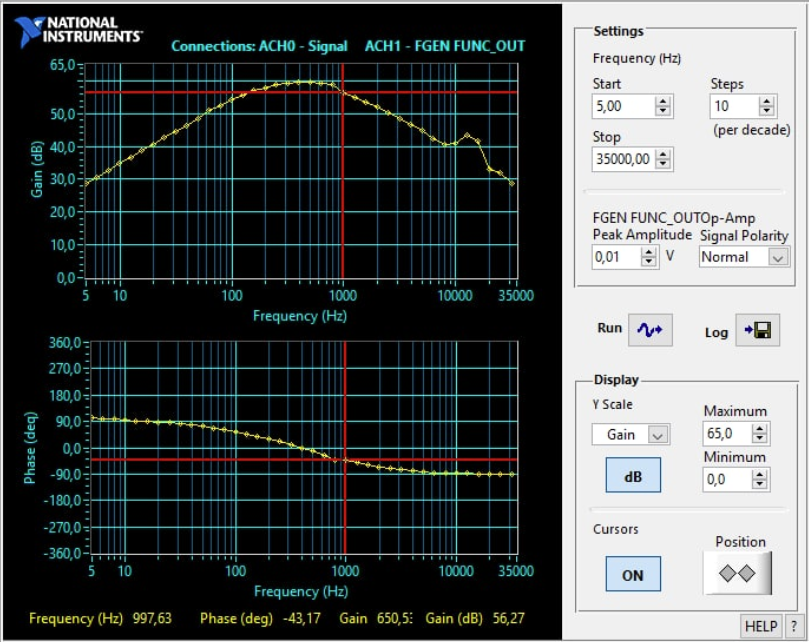
\includegraphics[width=0.7\linewidth]{photo/elvis_noninv}
	\caption{Частотная и фазовая характеристики усилителя на основе одного неинвертирующего РУ}
	\label{fig:elvis_noninv}
\end{figure}

\subsection{Усилитель на неинвертирующем и инвертирующем РУ}

Усилитель на инвертирующем и неинвертирующем РУ 
как раз обеспечивает достаточный коэффициент усиления, 
верхнюю и нижнюю граничную частоту. 
Такими образом, такой усилитель подходит 
под задание курсового проекта.

\begin{figure}[H]
	\centering
	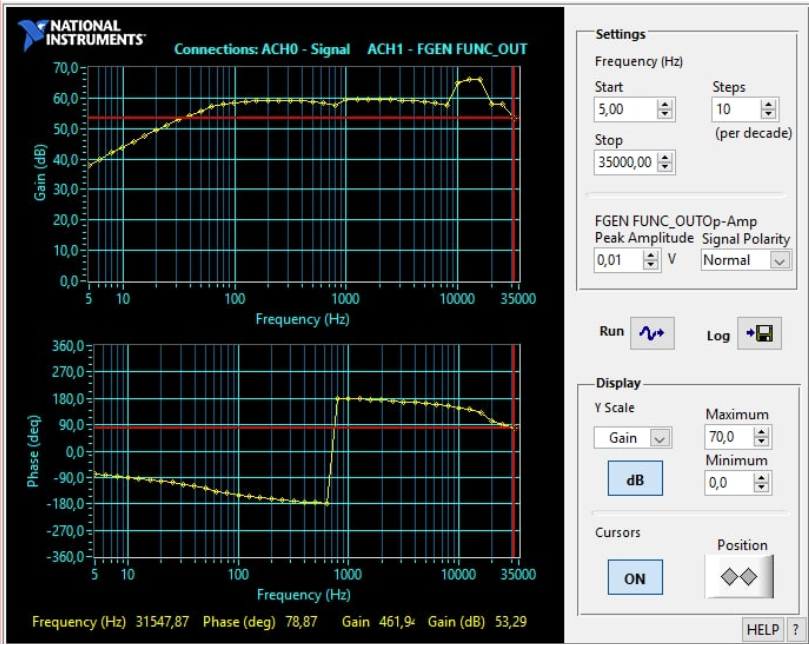
\includegraphics[width=0.7\linewidth]{photo/elvis_sub2}
	\caption{Частотная и фазовая характеристики усилителя на инвертирующем и неинвертирующем РУ}
	\label{fig:elvis_sub2}
\end{figure}

\subsection*{Вывод по исследованию усилителя переменного тока в системе \textit{NI ELVIS}}

ЛАЧХ данного усилителя переменного тока имеет большую,
чем у усилителя переменного тока на базе неинвертирующего РУ,
верхнюю граничную частоту, так как входная подсхема на базе
инвертирующего РУ позволяет обеспечить большее
входное сопротивление, а выходная на базе 
инвертирующего РУ – высокий коэффициент усиления всего усилителя.
Схема усилителя переменного тока на базе двух усилительных
подсхем позволяет обеспечить высокую верхнюю
граничную частоту при высоком коэффициенте усиления. 
